\documentclass{article}
\usepackage{tikz, pgfplots}
\usetikzlibrary{arrows}

\begin{document}
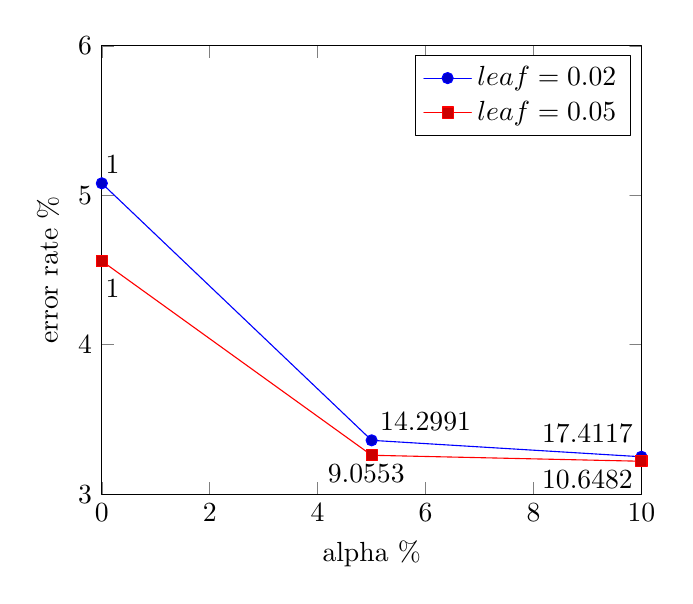
\begin{tikzpicture}[line cap=round,line join=round,>=triangle 45,x=1.0cm,y=1.0cm]
\begin{axis}[
xlabel=alpha \%,
xmin=0,
xmax=10,
ylabel=error rate \%,
ymin=3,
ymax=6]
\addplot coordinates{
(0,		5.08)
(5,	3.36)
(10,   3.25)
};
\addlegendentry{\(leaf=0.02\)};
\addplot coordinates{
(0,		4.56)
(5,	3.26)
(10,	3.22)
};
\addlegendentry{\(leaf=0.05\)};
\node[above]at(axis cs: 0.2,    5.08){\(1\)};
\node[above]at(axis cs: 6,    3.36){\(14.2991\)};
\node[above]at(axis cs: 9,    3.28){\(17.4117\)};
\node[below]at(axis cs: 0.2,    4.5){\(1\)};
\node[below]at(axis cs: 4.9,  3.26){\(9.0553\)};
\node[below]at(axis cs: 9,    3.22){\(10.6482\)};
\end{axis}
\end{tikzpicture}
\end{document}
